\documentclass[11pt,paper=letter]{scrartcl}
\usepackage[parskip]{cjquines}

\usepackage{tikz}
\usepackage{mathtools}
\usetikzlibrary{calc,intersections,through,angles,shapes.geometric}

\begin{document}

\title{PMO 2019 Qualifying Stage}
\author{Carl Joshua Quines}
\date{October 20, 2018}

\maketitle

The qualifying stage this year has become more difficult than the previous years. I'll present the questions and some solutions to all the problems. Are any explanations unclear? If so, contact me at \mailto{cj@cjquines.com}. More material is available on my website: \url{https://cjquines.com}.

\textbf{PART I.} Choose the best answer. Each correct answer is worth three points.

\begin{enumerate}[left=0pt]

\item The measures of the angles of a pentagon form an arithmetic sequence with common difference $15\dg$. Find the measure of the largest angle.

\fourch{$78\dg$}{$103\dg$}{$138\dg$}{$153\dg$}

\textbf{Answer:} $\boxed{\text{(c) }138\dg}$.

\textbf{Solution:} Suppose that the angles had measures $(a-30)\dg$, $(a-15)\dg$, $a\dg$, $(a+15)\dg$, and $(a+30)\dg$. Their sum is $5a\dg$, which must be equal to $540\dg$, hence $a = 108$. The largest angle is $108\dg + 30\dg = 138\dg$.

\item If $x - y = 4$ and $x^2 + y^2 = 5$, find the value of $x^3 - y^3$.

\fourch{$-24$}{$-2$}{$2$}{$8$}

\textbf{Answer:} $\boxed{\text{(b) }-2}$.

\textbf{Solution:} We know that $x^3 - y^3 = (x-y)(x^2 + xy + y^2)$, hence we need the value of $xy$. Squaring the first equation gives $x^2 - 2xy + y^2 = 16$. Combined with the second equation, we get $xy = -\dfrac{11}2$. Thus $$x^3 - y^3 = (x - y)(x^2 + y^2 + xy) = (4)\del{5 - \frac{11}2} = -2.$$

\item Five numbers are inserted between $4$ and $2916$ so that the resulting seven numbers form a geometric sequence. What is the fifth term of this geometric sequence?

\fourch{$324$}{$416$}{$584$}{$972$}

\textbf{Answer:} $\boxed{\text{(a) }324}$.

\textbf{Solution:} The first term of the sequence is $4$; let its common ratio be $r$. Note that $2916$ would be the seventh term of this geometric sequence, so by the formula for the $n$th term, we get $2916 = 4r^6$. Thus, $r = \pm 3$. The fifth term of the sequence is $4r^4 = 324$.

\item The constant term in the expansion of $\del{3x^2 - \dfrac1x}^6$ is

\fourch{$189$}{$135$}{$90$}{$54$}

\textbf{Answer:} $\boxed{\text{(b) }135}$.

\textbf{Solution:} We use the binomial theorem. The constant term is produced by $(x^2)^2\del{\dfrac1x}^4$. This gives the term as $$\binom{6}{2}(3x^2)^2\del{-\dfrac1x}^4 = 15(3)^2 = 135.$$

\item Juan has $4$ distinct jars and a certain number of identical balls. The number of ways that he can distribute the balls into the jars such that each jar has at least one ball is $56$. How many balls does he have?

\fourch{$9$}{$8$}{$7$}{$6$}

\textbf{Answer:} $\boxed{\text{(a) }9}$.

\textbf{Solution:} Consider lining up the $n$ balls in a row, and placing $3$ dividers in the $n-1$ spaces between them. These divide the $n$ balls into four groups, and counting the number of ways to do this is equivalent to the original problem. Since there are $n-1$ spaces in between and we choose $3$ of them as dividers, there are $\binom{n-1}{3}$ ways to do so. Setting $\binom{n-1}{3} = 56$ and solving, we get $n = 9$.

\textbf{Remark:} This is known as the balls-and-urns problem. We are distributing identical objects into distinct containers such that each container has at least one object. 

\item A regular octagon of area $48$ is inscribed in a circle. If a regular hexagon is inscribed in the same circle, what would its area be?

\fourch{$12\sqrt10$}{$18\sqrt6$}{$24\sqrt3$}{$30\sqrt2$}

\textbf{Answer:} $\boxed{\text{(b) }18\sqrt6}$.

\begin{center}
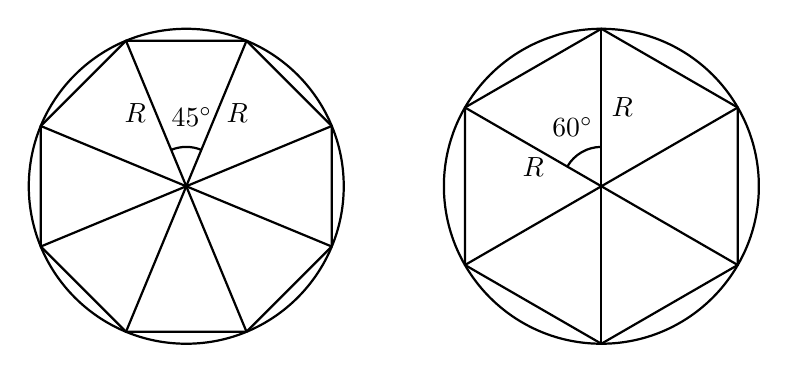
\begin{tikzpicture}[thick,scale=2]
\draw (0,0) circle (1);
\draw (22.5:1)--(67.5:1)--(112.5:1)--(157.5:1)--(202.5:1)--(247.5:1)--(292.5:1)--(337.5:1)--cycle;
\foreach \x in {22.5,67.5,...,337.5}{\draw (0,0)--(\x:1);}
\coordinate (O) at (0,0);
\coordinate (A) at (67.5:1);
\coordinate (B) at (112.5:1);
\node[right] at (67.5:.5){$R$};
\node[left] at (112.5:.5){$R$};
\draw pic[draw,pic text={$45^{\mathrlap{\circ}}$},angle eccentricity=1.75]{angle=A--O--B};
\begin{scope}[xshift=75]
\draw (0,0) circle (1);
\draw (30:1)--(90:1)--(150:1)--(210:1)--(270:1)--(330:1)--cycle;
\foreach \x in {30,90,...,330}{\draw (0,0)--(\x:1);}
\coordinate (O) at (0,0);
\coordinate (A) at (90:1);
\coordinate (B) at (150:1);
\node[right] at (90:.5){$R$};
\node[below] at (150:.5){$R$};
\draw pic[draw,pic text={$60^{\mathrlap{\circ}}$},angle eccentricity=1.75]{angle=A--O--B};
\end{scope}
\end{tikzpicture}
\end{center}
\textbf{Solution:} Let the radius of the circle be $r$. Draw the center of the circle, and connect it to each of the octagon's vertices. This creates eight congruent isosceles triangles with vertex angle $45\dg$. We know the area of a triangle with side lengths $a$ and $b$ and included angle $C$ is $\dfrac12 ab \sin C$. Thus the area of the octagon is $$8 \cdot \dfrac12 \cdot r^2 \sin 45\dg = 48,$$ and we get $r^2 = 12\sqrt2$. By similar reasoning, the area of the hexagon would be $$6 \cdot \dfrac12 \cdot r^2 \sin 60\dg = 18\sqrt6.$$

\item What is the smallest positive integer which when multiplied to $24^4 + 64$ makes the product a perfect square?

\fourch{$1037$}{$2074$}{$5185$}{$10370$}

\textbf{Answer:} $\boxed{\text{(c) }5185}$.

\textbf{Solution:} We use the Sophie-Germain factorization $a^4 + 4b^4 = \del{a^2 + 2b^2 + 2ab}\del{a^2 + 2b^2 - 2ab}$. It can be derived by completing the square like so: \begin{align*}
  a^4 + 4b^4 &= a^4 + 4a^2b^2 + 4b^4 - 4a^2b^2 \\
  &= (a^2 + 2b^2)^2 - (2ab)^2 \\
  &= (a^2 + 2b^2 + 2ab)(a^2 + 2b^2 - 2ab).
\end{align*} Here, we get \begin{align*}
24^4 + 4\cdot 2^4 &= (24^2 + 2\cdot 2^2 + 2\cdot 24 \cdot 2)(24^2 + 2 \cdot 2^2 - 2 \cdot 24 \cdot 2) \\
&= (680)(488) \\
&= (2^3 \cdot 5 \cdot 17)(2^3 \cdot 61) \\
&= 2^6 \cdot 5 \cdot 17 \cdot 61.
\end{align*} The prime factorization of a perfect square must have even exponents for each prime. To make the product a perfect square, we need to multiply by at least $5 \cdot 17 \cdot 61 = 5185$.

\item A bowl of negligible thickness is in the shape of a truncated circular cone, with height $4 \text{ in}$ and upper and lower radii of $9 \text{ in}$ and $6 \text{ in}$, respectively. What is the volume of the bowl? 

\fourch{$276\pi\text{ in}^3$}{$248\pi\text{ in}^3$}{$234\pi\text{ in}^3$}{$228\pi\text{ in}^3$}

\textbf{Answer:} $\boxed{\text{(d) }228\pi\text{ in}^3}$.

\textbf{Solution 1:} Extend the sides of the truncated cone to meet at the tip of the original cone. The volume is the difference of the volumes of two cones: the whole cone, and the cone that is truncated.
\begin{center}
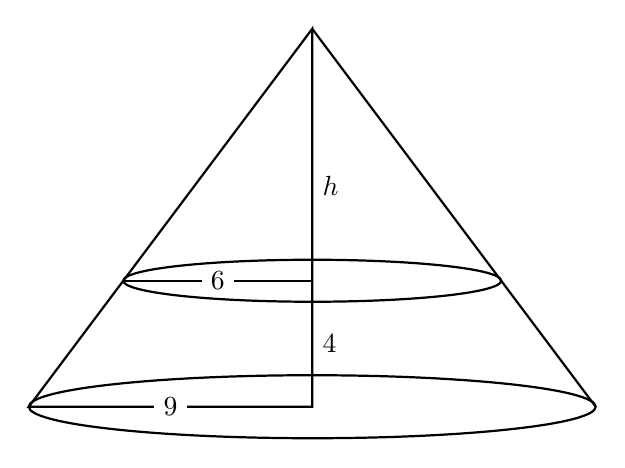
\begin{tikzpicture}[thick,scale=0.4]
\draw (-9,0)--(0,0)--(0,12)--cycle;
\draw (0,12)--(9,0);
\draw (-6,4)--(0,4);
\node[fill=white] at (-4.5,0) {9};
\node[fill=white] at (-3,4) {6};
\node[right] at (0,2) {4};
\node[right] at (0,7) {$h$};
\draw (0,0) ellipse (9 and 1);
\draw (0,4) ellipse (6 and 2/3);
\end{tikzpicture}
\end{center}

Consider the right triangle with legs $h$, the height of the truncated cone, and the radius $6$. This is similar to right triangle with legs $h + 4$, the height of the whole cone, and radius $9$. Since they are similar triangles, we get $$\frac{h}{6} = \frac{h+4}9,$$ and solving yields $h = 8$. 

The volume of a cone with height $h$ and radius $r$ is $\dfrac13\pi r^2h$. Thus the volume of the truncated cone is $$\frac13\pi\cdot9^2\cdot(8+4) - \frac13\pi\cdot6^2\cdot8 = 228\pi\text{ in}^3.$$

\textbf{Solution 2:} We use the formula $\dfrac{\pi h}3(R^2 + Rr + r^2)$, where $h$ is the height, and $R$ and $r$ are the upper and lower radii, respectively. This gives $228\pi\text{ in}^3$.

\textbf{Remark:} The formula in Solution 2 is derived through a similar solution in Solution 1.

\item A circle is tangent to the line $2x - y + 1 = 0$ at the point $(2, 5)$ and the center is on the line $x + y - 9 = 0$. Find the radius of the circle.

\fourch{$\sqrt{14}$}{$4$}{$3\sqrt2$}{$2\sqrt5$}

\textbf{Answer:} $\boxed{\text{(d) }2\sqrt5}$.

\textbf{Solution:} We know that the line joining the center of a circle to a point of tangency is perpendicular to the tangent line. Hence, the line perpendicular to $2x - y + 1 = 0$ and passing through $(2, 5)$ passes through the center of the circle. This is the line $x + 2y - 12 = 0$.

We are given the center also lies on $x + y - 9 = 0$. Solving the system of equations, we get the center as $(6, 3)$. Since $(2, 5)$ lies on the circumference of the circle, its radius must be the distance from the center $(6, 3)$ to the point $(2, 5)$. This is $\sqrt{(6-2)^2 + (3-5)^2} = 2\sqrt5$.

\item Suppose that $16$ points are drawn on a plane such that exactly $7$ of those points are collinear. Any set of three points which do not all belong to the $7$ are noncollinear. If $3$ random points are selected from the $16$ points, what is the probability that a triangle can be formed by joining those points?

\fourch{$\dfrac{15}{16}$}{$\dfrac{17}{20}$}{$\dfrac{19}{20}$}{$\dfrac{63}{80}$}

\textbf{Answer:} $\boxed{\text{(a) }\dfrac{15}{16}}$.

\textbf{Solution:} We will use complementary counting, and consider the probability a triangle \emph{cannot} be formed. A triangle cannot be formed only if the $3$ points chosen are among the $7$ collinear points, so there are $\binom73$ ways to do so. In total, there are $\binom{16}3$ ways to choose the points. Thus the probability we \emph{cannot} form a triangle is $$\frac{\binom73}{\binom{16}3} = \frac{7\cdot 6\cdot 5}{16 \cdot 15 \cdot 14} = \frac1{16}.$$ So the probability we \emph{can} form a triangle is $1 - \dfrac1{16} = \dfrac{15}{16}$.

\item The points $(0, -1)$, $(1, 1)$, and $(a, b)$ are distinct collinear points on the graph of $y^2 = x^3 - x + 1$. Find $a + b$.

\fourch{$-6$}{$-2$}{$1$}{$8$}

\textbf{Answer:} $\boxed{\text{(d) }8}$.

\textbf{Solution:} The line passing through the two points is $y = 2x - 1$. Substituting into the equation and simplifying, we get $x^3 - 4x^2 + 3x = 0$. We know that $x = 0$ and $x = 1$ are solutions of this (because they lie on both the line and the curve), hence we know $x(x-1)$ must be a factor. Indeed, the polynomial is $x(x-1)(x-3) = 0$, and the remaining point must have $x = 3$. Since it lies on $y = 2x - 1$, we get the point as $(3, 5)$, and $3+5 =8$. 

\textbf{Remark:} Curves of the form $y^2 = x^3 + ax + b$ for real numbers $a$ and $b$ are known as \emph{elliptic curves}. The problem describes collinear points on elliptic curves, which is how ``point addition'' is defined on them. A theorem about rational points on elliptic curves, called the \emph{modularity theorem}, is famously used to prove Fermat's Last Theorem.

\item What is the probability that a positive divisor of $2^{20}3^{17}$ also divides $2^83^6$?

\fourch{$\dfrac{12}{85}$}{$\dfrac29$}{$\dfrac19$}{$\dfrac16$}

\textbf{Answer:} $\boxed{\text{(d) }\dfrac16}$.

\textbf{Solution:} All divisors are of the form $2^a3^b$, where $0 \leq a \leq 20$ and $0 \leq b \leq 17$ are integers. For this to also be a divisor of $2^83^6$, we must have $a \leq 8$ and $b \leq 6$. Thus the possible choices for $a$ are $0, 1, \ldots, 8$ out of $0, 1, \ldots, 20$, for a probability of $\dfrac{9}{21}$. Similarly, the probability that $b$ satisfies the condition is $\dfrac{7}{18}$. Multiplying, since we want both $a$ and $b$ to satisfy the condition, we get $\dfrac{9}{21} \cdot \dfrac{7}{18} = \dfrac16$.

\item Let $ABC$ be a right triangle where $AB = 7$, $BC = 24$, and with hypotenuse $AC$. Point $D$ is on $AC$ such that $AD : DC = 2 : 3$. Let $m$ and $n$ be the relative prime positive integers such that $BD^2 = \frac mn$. What is $m + n$?

\fourch{$554$}{$550$}{$544$}{$540$}

\textbf{Answer:} $\boxed{\text{(a) }554}$.

\textbf{Solution 1:} Let the foot of the perpendiculars from $D$ to $AB$ and $BC$ and be $E$ and $F$, respectively. Then triangles $AED$ and $ABC$ are similar with the ratio $2 : 5$, so $ED = \dfrac25 BC = \dfrac{48}5$. Also, triangles $DFC$ and $ABC$ are similar with the ratio $3 : 5$, so $DF = \dfrac35 AB = \dfrac{21}5$. 
\begin{center}
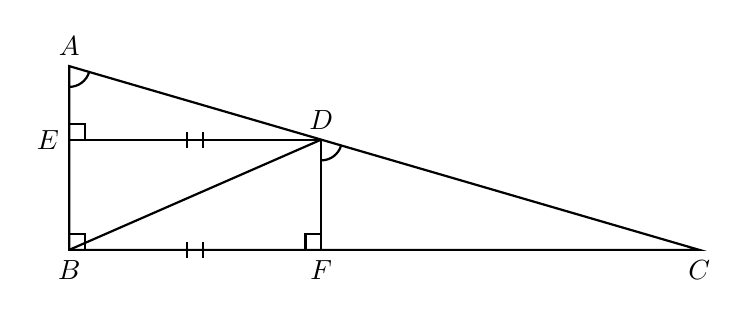
\begin{tikzpicture}[thick,scale=1/3]
\draw (0,0) node[below]{$B$} coordinate(B)--(24,0) node[below]{$C$} coordinate(C)--(0,7) node[above]{$A$} coordinate(A)--cycle;
\draw (0,21/5) node[left] {$E$} coordinate(E)--(48/5,21/5) node[above]{$D$} coordinate(D)--(48/5,0) node[below]{$F$} coordinate(F);
\draw (B)--(D);
\draw pic[draw,angle radius=7.5]{angle=E--A--D} pic[draw, angle radius=7.5]{angle=F--D--C};
\node at ( $(B)!.5!(F)$ ) {\tikz[thick]{\draw (-.1,-.1)--(-.1,.1) (.1,-.1)--(.1,.1);}};
\node at ( $(E)!.5!(D)$ ) {\tikz[thick]{\draw (-.1,-.1)--(-.1,.1) (.1,-.1)--(.1,.1);}};
\draw (3/5,21/5)|-(0,24/5);
\draw (3/5,0)|-(0,3/5);
\draw (48/5,3/5)-|(9,0);
\end{tikzpicture}
\end{center}

Note that $EDFB$ is a rectangle, so $ED = FB = \dfrac{48}5$. By the Pythagorean theorem on right triangle $DFB$, $$BD^2 = DF^2 + FB^2 = \del{\dfrac{21}5}^2 + \del{\dfrac{48}5}^2 = \dfrac{2745}{25} = \dfrac{549}5,$$ so the answer is $549 + 5 = 554$.

\textbf{Solution 2:} We use coordinates. Set $A(0, 7)$, $B(0, 0)$, $C(24, 0)$.
\begin{center}
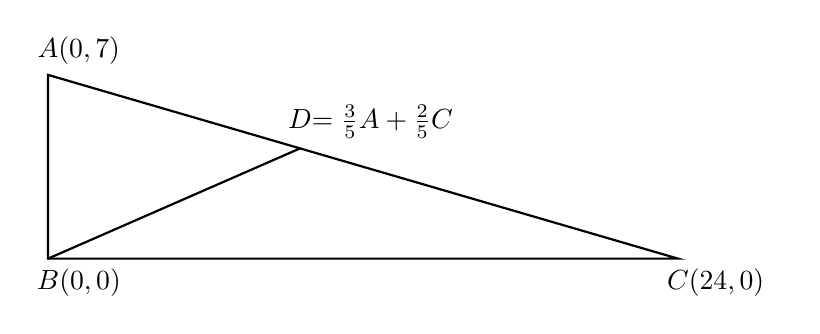
\begin{tikzpicture}[thick,scale=1/3]
\draw (0,0) node[below]{$B\mathrlap{(0,0)}$} coordinate(B)--(24,0) node[below]{$C\mathrlap{(24,0)}$} coordinate(C)--(0,7) node[above]{$A\mathrlap{(0,7)}$} coordinate(A)--cycle;
\node at (28,0){};
\draw (B)--(48/5,21/5) node[above]{$D\mathrlap{=\frac35A+\frac25C}$};
\end{tikzpicture}
\end{center}
Since $AD : DC = 2 : 3$, we must have $D = \dfrac35A + \dfrac25C$, in terms of coordinates. To see this, we can use the well-known formula or similar triangles, as above. Here, we will use vectors.

Note that $\vec{D}$ is $\dfrac25$ of the way from $\vec{A}$ on $\vec{AC}$. Hence $\vec{D} = \vec{A} + \dfrac25\vec{AC} = \vec{A} + \dfrac25\del{\vec{C} - \vec{A}} = \dfrac35\vec{A} + \dfrac25\vec{C}$. Using this, we can solve the coordinates of $D$ as $\del{\dfrac35 \cdot 0 + \dfrac25 \cdot 24, \dfrac35 \cdot 7 + \dfrac25 \cdot 0} = \del{\dfrac{48}5, \dfrac{21}5}$. Using the Pythagorean Theorem to find the distance we get $\dfrac{549}5$, so the answer is $549 + 5 = 554$.

\textbf{Solution 3:} By the Pythagorean theorem, $AC = 25$, hence $AD = 10$ and $DC = 15$. By Stewart's Theorem, \begin{align*}
AD \cdot AC \cdot DC + BD^2 \cdot AC &= BC^2 \cdot AD + AB^2 \cdot DC \\
(10)(25)(15) + BD^2(25) &= (24^2)(10) + (7^2)(15) \\
25BD^2 &= 2745,
\end{align*}so $BD^2 = \dfrac{549}{5}$ and the answer is $549 + 5 = 554$.

\item In chess, a knight moves by initially taking two steps in any horizontal or vertical direction and then taking one more step in any direction that is perpendicular to its initial movement. Suppose Renzo places a knight on a random tile on an $8 \times 8$ chessboard. Find the probability that he can land on a corner tile in exactly two moves.

\fourch{$\dfrac3{16}$}{$\dfrac14$}{$\dfrac9{16}$}{$\dfrac58$}

\textbf{Answer:} $\boxed{\text{(d) }\dfrac58}$.

\textbf{Solution:} It is easier to solve the problem backwards. Beginning from the corners, we count the number of squares that can be reached in exactly two moves. We can do this by drawing a diagram:
\begin{center}
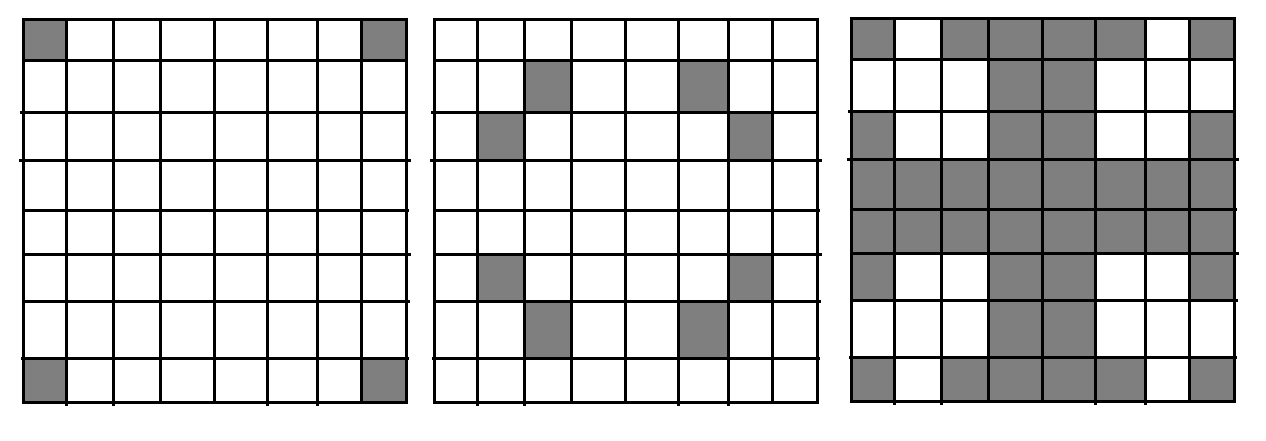
\includegraphics[width=5in]{291.png}
\end{center}
From left to right are the number of possible squares that can be reached from the corners with zero, one, and two moves. There are $40$ possible squares that can be reached from the corners in two moves, so there are $40$ possible squares that can reach the corners in two moves. This gives the probability as $\dfrac{40}{64} = \dfrac58$.

\item In rectangle $ABCD$, point $Q$ lies on side $AB$ such that $AQ : QB = 1 : 2$. Ray $CQ$ is extended past $Q$ to $R$ so that $AR$ is parallel to $BD$. If the area of triangle $ARQ$ is $4$, what is the area of rectangle $ABCD$?

\fourch{$108$}{$120$}{$132$}{$144$}

\textbf{Answer:} $\boxed{\text{(b) }120}$.

\newpage

\textbf{Solution 1:} Let $BD$ and $CQ$ intersect at point $S$. Triangles $ARQ$ and $BSQ$ are similar in the ratio $1 : 2$, hence their areas are in the ratio $1 : 4$, and the area of $BSQ$ is $16$. We now try to relate the area of triangle $BSQ$ to the area of triangle $ADB$. To do this, we find the ratios of their heights and their bases.
\begin{center}
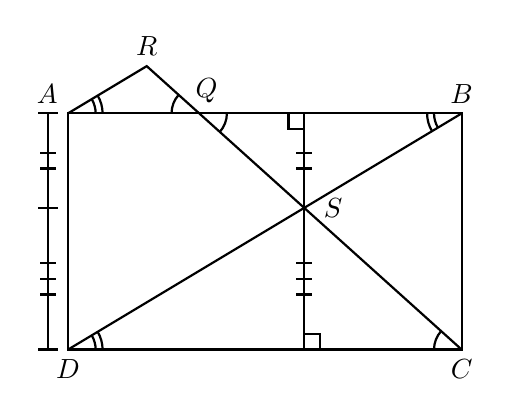
\begin{tikzpicture}[thick,scale=.5]
\draw (0,0) node[below]{$D$} coordinate(D)--(10,0) node[below]{$C$} coordinate(C)--(10,6) node[above]{$B$} coordinate(B)--(0,6) node[above left]{$A$} coordinate(A)--cycle;
\draw (B)--(D);
\draw (C)--(2,36/5) node[above]{$R$} coordinate(R)--(A);
\draw (-.5,0)--(-.5,6);
\draw (6,0)--(6,6);
\draw (10/3,6) coordinate(Q) node[above right]{$\!\!\!Q$} (6,18/5) node[right]{$\ S$} coordinate(S);
\foreach \y in {0,18/5,6}{\draw (-.75,\y)--(-.25,\y);}
\node at ( $(-.5,6)!.5!(-.5,18/5)$ ) {\tikz[thick]{\draw (-.1,.1)--(.1,.1) (-.1,-.1)--(.1,-.1);}};
\node at ( $(-.5,0)!.5!(-.5,18/5)$ ) {\tikz[thick]{\draw (-.1,.2)--(.1,.2) (-.1,-.2)--(.1,-.2) (-.1,0)--(.1,0);}};
\node at ( $(6,6)!.5!(6,18/5)$ ) {\tikz[thick]{\draw (-.1,.1)--(.1,.1) (-.1,-.1)--(.1,-.1);}};
\node at ( $(6,0)!.5!(6,18/5)$ ) {\tikz[thick]{\draw (-.1,.2)--(.1,.2) (-.1,-.2)--(.1,-.2) (-.1,0)--(.1,0);}};
\draw pic[draw,angle radius=10]{angle=R--Q--A} pic[draw,angle radius=10]{angle=C--Q--B} pic[draw,angle radius=10]{angle=Q--C--D};
\draw pic[draw,angle radius=10]{angle=Q--A--R} pic[draw,angle radius=12.5]{angle=Q--A--R} pic[draw,angle radius=10]{angle=A--B--D} pic[draw,angle radius=12.5]{angle=A--B--D} pic[draw,angle radius=10]{angle=C--D--B} pic[draw,angle radius=12.5]{angle=C--D--B};
\draw (6,28/5)-|(28/5,6) (6,2/5)-|(32/5,0);
\end{tikzpicture}
\end{center}

Triangle $BSQ$ is similar to triangle $DSC$ in the ratio $2 : 3$. Hence their heights must be in the ratio $2 : 3$. Hence the height from $S$ to $QB$ and the height from $S$ to $DC$ are in the ratio $2 : 3$. But, in total, they form the length $AD$. Thus the height from $S$ to $QB$ and the side $AD$ are in the ratio $2 : 5$.

But $QB : AB = 2 : 3$. So the areas of $BSQ$ and $ADB$ are in the ratio $2 \cdot 2 : 3 \cdot 5$, or $4 : 15$. Hence the area of $ADB$ is $60$, making the area of the rectangle $120$.

\textbf{Solution 2:} Knowing the answer is numerical, and that we only care about the ratios of areas, we can choose $ABCD$ to be a square of side length $3$. We also use coordinates. Set $A(0, 3)$, $B(3, 3)$, $C(3, 0)$, and $D(0, 0)$. This gives $Q(1, 3)$.

The slope of $BD$ is $1$, so the line through $A$ parallel to $BD$ is $y - x - 3 = 0$. The line $CQ$ can be solved as $3x + 2y - 9 = 0$. Intersecting them gives $R\del{\dfrac35, \dfrac{18}5}$. We can see the distance from $R$ to $AQ$ is $\dfrac{18}5 - 3 = \dfrac35$, and since $AQ = 1$, its area is $\dfrac3{10}$. Thus the ratio of areas of $ARQ$ to $ABCD$ is $\dfrac3{10} : 9$. Since its actual area is $4$, the area of $ABCD$ must be $120$.
\begin{center}
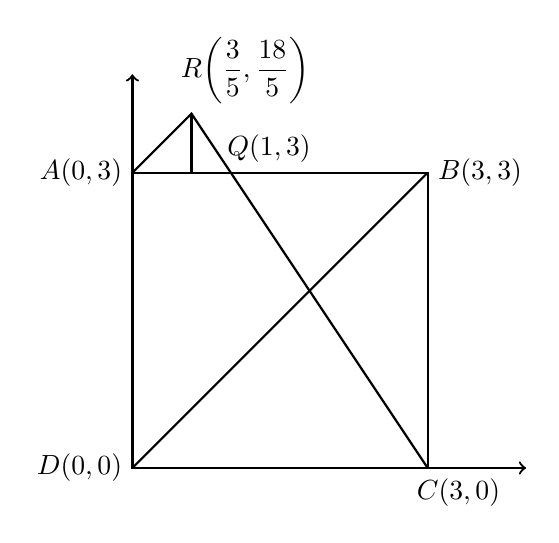
\begin{tikzpicture}[thick,scale=1.25]
\draw[<->] (4,0)-|(0,4);
\draw (0,0) node[left]{$D(0,0)$};
\draw (3,0) node[below]{$C\mathrlap{(3,0)}$}--(3,3) node[right]{$B(3,3)$}--(0,3) node[left]{$A(0,3)$};
\draw (0,0)--(3,3);
\draw (0,3)--(3/5,18/5) node[above]{$R\mathrlap{\left(\dfrac35,\dfrac{18}{5}\right)}$}--(3,0);
\node[above right] at (1,3) {$\!\!\!Q\mathrlap{(1,3)}$};
\draw (3/5,18/5)--(3/5,3);
\end{tikzpicture}
\end{center}

\textbf{Remark:} Solution 2 can be justified as follows. Imagine compressing the plane horizontally until $ABCD$ becomes a square. The ratios of the areas do not change, the ratios of points on a line do not change, and neither do parallel lines. Also, you can scale $ABCD$ such that its side length is $3$, and again, the ratios of the areas do not change again.

Scaling and compressing are both examples of \emph{affine transformations}, which preserve parallel lines, ratios of areas, and ratios of distances between points on a line. Affine transformations make solving problems like these much easier.

\end{enumerate}

\noindent\textbf{PART II.} Choose the best answer. Each correct answer is worth three points.

\begin{enumerate}[left=0pt]

\item How many two-digit numbers are there such that the product of their digits is equal to a prime raised to a positive integer exponent?

\fourch{$27$}{$28$}{$29$}{$30$}

\textbf{Answer:} $\boxed{\text{(c) }29}$.

\textbf{Solution:} Since the digits are single-digit numbers, the prime must be a single-digit number as well. Thus it is either $2$, $3$, $5$, or $7$.

In the case of $2$, the digits could be any of $1$, $2$, $4$, or $8$. This gives $4^2 = 16$ possibilities. We must exclude the case $1 \cdot 1$, so there are $15$ possibilities.

Similarly, in the case of $3$, the digits could be any of $1$, $3$, or $9$. This gives $3^2 = 9$ possibilities. Excluding the case $1 \cdot 1$, we get $8$ possibilities.

Similarly, for $5$ and $7$, we get $2^2 - 1 = 3$ possibilities each. This gives a total of $15 + 8 + 3 + 3 = 29$ possibilities in all.

\item $ABCDEF$ is a six-digit perfect square in base $10$ such that $DEF = 8 \times ABC$. What is $A + B + C+ D + E + F$? (Note that $ABCDEF$, $ABC$, and $DEF$ should be interpreted as numerals in base $10$ and not as products of digits.)

\fourch{$18$}{$27$}{$36$}{$45$}

\textbf{Answer:} $\boxed{\text{(b) }27}$.

\textbf{Solution:} Note that the number is $1000 \cdot ABC + DEF$, or $1000 \cdot ABC + 8 \cdot ABC$, or $1008 \cdot ABC$. Observe that $1008 = 2^4 \cdot 3^2 \cdot 7$.

Since the exponents in the prime factorization of a perfect square must all be even, $ABC$ must be $7$ times a perfect square. Since $ABC$ is a three-digit number, it must be at least $100$. Since $DEF$ is a three-digit number, $ABC$ must at most $\dfrac{1000}{8} = 125$. The only possibility is $7 \cdot 16 = 112$, making the perfect square $112896$, with digit sum $27$.

\item Quadrilateral $ABCD$ has $AB = 25$, $BC = 60$, $CD = 39$, $DA = 52$, and $AC = 65$. What is the inradius of $\triangle BCD$?

\fourch{$14$}{$15$}{$16$}{$18$}

\textbf{Answer:} $\boxed{\text{(a) }14}$.

\textbf{Solution 1:} We note that triangle $ABC$ has side lengths $25$, $60$, and $65$. Thus, it is similar to the triangle with side lengths $5$, $12$, and $13$, which is a right triangle. So triangle $ABC$ is right with $\angle ABC = 90\dg$. Similarly, triangle $CDA$ is similar to a 3-4-5 right triangle, so $\angle CDA = 90\dg$. 
\begin{center}
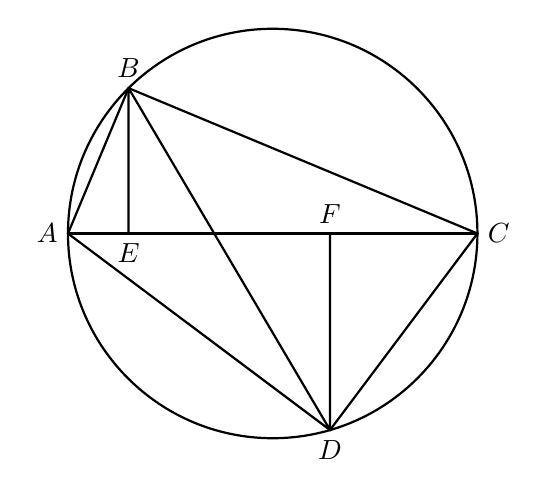
\begin{tikzpicture}[thick,scale=0.2]
\draw (0,0) circle (13);
\draw (-13,0) node[left]{$A$}--(13,0) node[right]{$C$};
\draw (-13,0)--( {2*asin(12/13)}:13) node[above]{$B$} coordinate(B)--(13,0)--( {2*asin(-3/5)}:13) node[below]{$D$} coordinate(D)--cycle;
\draw ( {13*cos(2*asin(12/13))},0) node[below]{$E$}--(B) (B)--(D) (D)--( {13*cos(2*asin(-3/5))},0) node[above]{$F$};
\end{tikzpicture}
\end{center}
Drop perpendiculars $E$ and $F$ to $AC$ from $B$ and $D$, respectively. Since $\triangle AEB \sim \triangle ABC$, $AE = AB \cdot \dfrac{AB}{AC} = \dfrac{125}{13}$ and $BE = AB \cdot \dfrac{BC}{AC} = \dfrac{300}{13}$. Similarly, because $\triangle DFA \sim \triangle CDA$, $AF = DA \cdot \dfrac{DA}{AC} = \dfrac{208}5$ and $DF = AD \cdot \dfrac{CD}{AC} = \dfrac{156}5$.

By the Pythagorean Theorem, $BD^2 = (BE + FD)^2 + EF^2 = (BE + FD)^2 + (AF - AE)^2 = 3969$, so $BD = 63$. By Heron's theorem, the area of $BCD$ is $$\sqrt{81(81 - 63)(81 - 60)(81 - 39)} = \sqrt{81 \cdot 18 \cdot 21 \cdot 42} = 1134.$$ But since the area is also the semiperimeter times the inradius, the inradius must be $\dfrac{1134}{81} = 14$.

\textbf{Solution 2:} By the previous solution, we know that $\angle ABC = \angle CDA = 90\dg$. Thus, the circumcircle of triangle $ABC$ has diameter $AC$, and so does the circumcircle of triangle $CDA$. So they must share the same circumcircle; in other words, quadrilateral $ABCD$ is cyclic. We can also get this from the fact $\angle ABC + \angle CDA = 180\dg$.

Since $ABCD$ is cyclic, by Ptolemy's theorem, \begin{align*}
AB \cdot CD + BC \cdot DA &= AC \cdot BD \\
(25)(39) + (60)(52) &= (65)BD \\
BD &= 63.\end{align*} Then a similar solution to the above can be used.

\item Find the sum of the first $20$ positive integers that are multiples of either $3$ or $7$ but not both.

\fourch{$336$}{$399$}{$529$}{$592$}

\textbf{Answer:} $\boxed{\text{(c) }529}$.

\textbf{Solution:} We first estimate the largest integer among them. Suppose the largest integer is $n$. Then the number of integers less than or equal to $n$ that are multiples of $3$ or $7$ but not both, by PIE, is $$
20 = \floor{\frac n3} + \floor{\frac n7} - 2\floor{\frac n{21}} \\
 \approx \frac n3 + \frac n7 - 2\frac n{21} \\
 \approx \frac {8n}{21},
$$
so $n$ is about $52.5$. Checking, we see $n = 52$ satisfies the first equation, so $52$ is an upper bound. 

Summing the multiples of $3$ less than $52$ gives $$3 + 6 + \cdots + 51 = 3(1 + 2 + \cdots + 17) = 3\cdot \dfrac{(17)(18)}2 = 459.$$ Summing the multiples of $7$ less than $52$ gives $$7 + 14 + \cdots + 49 = 7(1 + 2 + \cdots + 7) = 196.$$ The multiples of $21$ less than $52$ are $21$ and $42$, with sum $63$. Hence the total sum is $459 + 196 - 2(63) = 529$.

\item $Q$ is a rational function with $xQ(x + 2018) = (x - 2018)Q(x)$ for all $x \not\in \cbr{0, 2018}$. If $Q(1) = 1$, what is $Q(2017)$?

\fourch{$2020$}{$2019$}{$2018$}{$2017$}

\textbf{Answer:} $\boxed{\text{(d) }2017}$.

\textbf{Solution 1:} By repeatedly substituting $x+2018$ for $x$, we get $$(x-2018)Q(x) = xQ(x+2018) = (x+2018)Q(x+4036) = (x+4036)Q(x+6054) = \cdots.$$
Let $R(x) = (x-2018)Q(x) + 2017$. By the above, we see it is equal to $0$ for all of $1$, $1+2018$, $1+4036$, and so on. Hence, it must be the zero function. Solving, we get $Q(x) = -\dfrac{2017}{x-2018}$, and thus $Q(2017) = 2017$.

\textbf{Solution 2:} Since the answer is numerical, any rational function $Q$ that satisfies the conditions should give the right answer. We see the $x-2018$ multiplied on the right-hand side, and wanting to cancel it out, try that as the denominator. 

We try $Q(x) = \dfrac1{x-2018}$. This satisfies the equation, but does not satisfy $Q(1) = 1$, so we multiply it by $-2017$. We get $Q(x) = -\dfrac{2017}{x-2018}$, which satisfies all the conditions. Then $Q(2017) = 2017$.

\item How many ordered pairs $(x, y)$ of positive integers are there such that $1 \leq x \leq y \leq 20$ and both $\dfrac yx$ and $\dfrac{y+2}{x+2}$ are integers?

\fourch{$38$}{$36$}{$34$}{$32$}

\textbf{Answer:} $\boxed{\text{(d) }32}$.

\textbf{Solution:} Since $\dfrac yx$ and $\dfrac{y+2}{x+2}$ are integers, then $\dfrac yx - 1$ and $\dfrac{y+2}{x+2} - 1$ are both integers as well. But these are $\dfrac{y-x}x$ and $\dfrac{y-x}{x+2}$, so $y-x$ is divisible by both $x$ and $x+2$.

We first note that $y = x$ is always a solution, so we only deal with the case $y > x$:
\begin{itemize}
  \item If $x = 1$, then $y-x$ is divisible by $1$ and $3$, or by $3$. Then $y-x$ can be $3, 6, \ldots 18$: $6$ pairs.
  \item If $x = 2$, then $y-x$ is divisible by $2$ and $4$, or by $4$. Then $y-x$ can be $4, 8, 12, 16$: $4$ pairs.
  \item If $x = 3$, then $y-x$ is divisible by $3$ and $5$, or by $15$. Then $y-x$ can only be $15$: $1$ pair.
  \item If $x = 4$, then $y-x$ is divisible by $4$ and $6$, or by $12$. Then $y-x$ can only be $12$: $1$ pair.
  \item No larger choice of $x$ is possible, because $y-x$ would have to be too large.
\end{itemize}
This gives a total of $20 + 6 + 4 + 1 + 1 = 32$ pairs.

\textbf{Remark:} Note that $$\dfrac yx - \dfrac{y+2}{x+2}= \dfrac{2(y-x)}{x(x+2)}$$ must be an integer, so $2(y-x)$ is divisible by both $x$ and $x+2$. After this, a similar solution to the above works. It is also possible to write a solution using a bounding argument. 

\item An entertainment agency has seven trainees. Each of the trainees does at least one of dancing, singing, and rapping, and no two trainees have the same skill set. How many ways can the agency choose three trainees to form a group, provided that the group must have at least one dancer, one singer, and one rapper (who are not necessarily distinct)?

\fourch{$26$}{$29$}{$32$}{$35$}

\textbf{Answer:} $\boxed{\text{(c) }32}$.

\textbf{Solution:} We use complementary counting and count the number of ways their group \emph{does not} have a dancer, singer, or rapper. Suppose that no one in a group can dance. Then the only possible skill sets are $\cbr{\text{singer}}$, $\cbr{\text{rapper}}$, and $\cbr{\text{singer}, \text{rapper}}$. By the conditions in the problem, the group must consist of these three people, and there is only $1$ group.

Similarly, there is only $1$ possible group where no one is a singer, and only $1$ possible group where no one is a rapper. It can be seen that these groups are all different. This makes $3$ ways for a group to \emph{not} have a dancer, singer, or rapper. There are $\binom73 = 35$ ways to choose in total, and subtracting $3$ ways that do not work give $32$ remaining ways.

\item Let $\triangle ABC$ be a right triangle such that its hypotenuse $AC$ has length $10$ and $\angle BAC = 15\dg$. Let $O$ be the center of the circumcircle of $\triangle ABC$. Let $E$ be the point of intersection of the lines tangent to the circumcircle at points $A$ and $B$, and $F$ be the point of intersection of the lines tangent to the circumcircle at points $B$ and $C$. The area of $\triangle OEF$ is

\fourch{$\dfrac{25}8$}{$50$}{$100$}{$\dfrac{225}8$}

\textbf{Answer:} $\boxed{\text{(b) }50}$.

\begin{center}
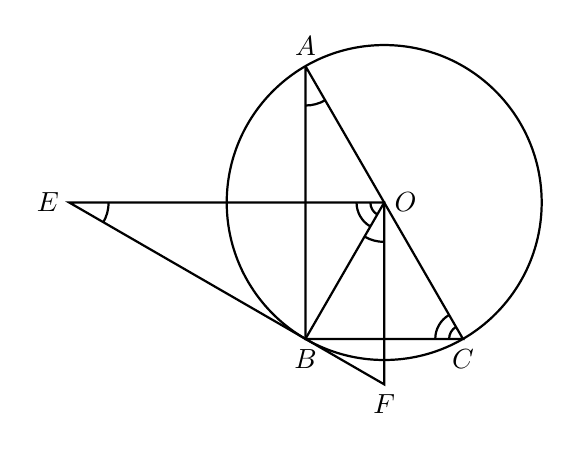
\begin{tikzpicture}[thick,scale=0.4]
\draw (0,0) node[right]{$O$} coordinate(O) circle (5);
\draw (120:5) node[above]{$A$} coordinate(A)--(300:5) node[below]{$C$} coordinate(C)--(240:5) node[below]{$B$} coordinate(B)--(120:5);
\draw (O)--(B);
\draw ( {-5/sin(30)},0) node[left]{$E$} coordinate(E)--(O)--(0,{-5/sin(60)} ) node[below]{$F$} coordinate(F)--cycle;
\draw pic[draw]{angle=B--A--C} pic[draw]{angle=B--E--O} pic[draw]{angle=B--O--F};
\draw pic[draw,angle radius=5]{angle=E--O--B} pic[draw,angle radius=10]{angle=E--O--B};
\draw pic[draw,angle radius=5]{angle=A--C--B} pic[draw,angle radius=10]{angle=A--C--B};
\end{tikzpicture}
\end{center}
\textbf{Solution:} It is well-known that $O$ is the midpoint of $AC$. Observe that triangles $EBO$, $ABC$, and $OBF$ are similar: they share right angles $\angle EBO$ and $\angle OBF$ due to tangent lines, and it can be shown that the other angles are congruent. But $\angle EOF = \angle EOB + \angle BOF = 15\dg + 75\dg = 90\dg,$ so the area of triangle $OEF$ is $$
\frac12 \cdot OE \cdot OF = \frac12 \cdot \frac{AC\cdot BO}{BC} \cdot \frac{AC \cdot BO}{AB} = \frac{AC^2 \cdot BO^2}{2 \cdot AC \sin 15\dg \cdot AC \cos 15\dg} = \frac{BO^2}{\sin 30\dg} = \frac{5^2}{\frac12} = 50.
$$
From left-to-right, we apply similar triangles, use the fact that $\angle ACB = 15\dg$, and then use the double-angle formula. 

\textbf{Remark:} The figure provided is not to scale. There are many other ways to solve this problem that use the same observations. It is possible to use the values of $\sin 15\dg$ and $\cos 15\dg$ to solve this problem: one can memorize them, or derive them from the half-angle formula. Here is a hint for a synthetic way to derive their values: let $D$ be the point on side $BC$ such that $\angle BAD = 60\dg$, then triangle $BAD$ is 30-60-90, and triangle $ADC$ is isosceles. 

\item A real number $x$ is chosen randomly from the interval $(0, 1)$. What is the probability that $\floor{\log_5(3x)} = \floor{\log_5 x}$? (Here, $\floor{x}$ denotes the greatest integer less than or equal to $x$.)

\fourch{$\dfrac16$}{$\dfrac5{36}$}{$\dfrac19$}{$\dfrac1{12}$}

\textbf{Answer:} $\boxed{\text{(a) }\dfrac16}$.

\textbf{Solution:} Fix $n = \floor{\log_5 x}$; we find the probability that $n$ is also $\floor{\log_5(3x)}$.  For $n = \floor{\log_5 x}$, we need $n \leq \log_5 x < n+1$, or $x \in [5^n, 5^{n+1})$.

For $n = \floor{\log_5(3x)}$ to be true, we need $5^n \leq 3x < 5^{n+1}$ to be true as well. It is clear that $3x \geq 5^n$ is already true for all $x \in [5^n, 5^{n+1})$. We need to be true $x < \dfrac{5^{n+1}}3$, or $x \in \left[5^n, \dfrac{5^{n+1}}3\right)$.

To find the probability, we find the lengths of the intervals and divide them. This gives $$\frac{\frac{5^{n+1}}3 - 5^n}{5^{n+1} - 5^n} = \frac{5^n}{5^n} \cdot \frac{\frac53 - 1}{5 - 1} = \frac16.$$ Since it does not depend on $n$, the total probability is also $\dfrac16$.

\textbf{Remark:} Compare to AMC 12B 2006/20: \emph{Let $x$ be chosen at random from the interval $(0, 1)$. What is the probability that $\floor{\log_{10} 4x} - \floor{\log_{10} x} = 0$?}

\item What is the remainder when $1^{2018} + 2^{2018} + \cdots + 2017^{2018}$ is divided by $2018$?

\fourch{$0$}{$2$}{$1009$}{$2017$}

\textbf{Answer:} $\boxed{\text{(c) }1009}$.

\textbf{Solution 1:} We note that $2018$ factorizes as $2 \cdot 1009$. We will evaluate the sum modulo $2$ and modulo $1009$, and combine the results to get the sum modulo $2018$.

Modulo $2$, the sum is $$1^{2018} + 0^{2018} + \cdots + 1^{2018} \equiv 1 + 0 + \cdots + 1 \equiv 1.$$ Modulo $1009$, the sum is $$1^{2018} + 2^{2018} + \cdots + 1008^{2018} + 0^{2018} + 1^{2018} + \cdots + 1008^{2018} \equiv 2\del{1^{2018} + 2^{2018} + \cdots + 1008^{2018}}.$$ By Fermat's little theorem, $a^{2018} \equiv \del{a^{1008}}^2 \cdot a^2 \equiv 1^2 \cdot a^2 \equiv a^2$ for any $a \not\equiv 0$. So by the formula for the sum of squares, the sum is $$2\del{1^2 + 2^2 + \ldots + 1008^2} \equiv 2 \cdot \frac{(1008)(1009)(2017)}6 \equiv 1009 \cdot \frac{(1008)(2017)}3 \equiv 0.$$ Since the sum is $1$ modulo $2$ and $0$ modulo $1009$, the whole sum must be $1009$ modulo $2018$.

\textbf{Solution 2:} Here is an alternative way to evaluate the sum modulo $1009$. Let $g$ be a primitive root. Then the set $\cbr{1, 2, \ldots, 1008}$ is the same set as $\cbr{1, g, g^2, \ldots, g^{1007}}$, by definition of a primitive root. The sum is $$2\del{1 + g^{2018} + g^{(2)(2018)} + \cdots + g^{(1007)(2018)}} \equiv 2 \cdot \frac{g^{(1008)(2018)} - 1}{g^{2018} - 1} \equiv 0$$ by Fermat's little theorem.

\textbf{Remark:} The same method in Solution 2 shows the following well-known lemma: let $p$ be a prime and $m$ an integer not divisible by $p-1$. Then $1^m + 2^m + \cdots + (p-1)^m$ is divisible by $p$. It works even when $m$ is negative.

\end{enumerate}

\noindent\textbf{PART III.} All answers should be in simplest form. Each correct answer is worth six points.

\begin{enumerate}[left=0pt]

\item Suppose two numbers are randomly selected in order, and without replacement, from the set $\cbr{1, 2, 3, \ldots, 888}$. Find the probability that the difference of their squares is not divisible by $8$.

\textbf{Answer:} $\boxed{\dfrac{555}{887}}$.

\textbf{Solution:} The square of a number modulo $8$ can be either $0$, if it is divisible by $4$; $1$, if it is odd; or $4$, if it $2$ modulo $4$.

We will use complementary counting and determine the probability it \emph{is} divisible by $8$. Note that the difference can only be $0$ modulo $8$ if their squares are the same modulo $8$. Thus we are looking for the probability that the two numbers chosen are both:
\begin{itemize}
  \item divisible by $4$, with probability $\dfrac{222}{888} \cdot \dfrac{221}{887} = \dfrac{221}{3548}$,
  \item odd, with probability $\dfrac{444}{888} \cdot \dfrac{443}{887} = \dfrac{886}{3548}$,
  \item or $2$ modulo $4$, with probability $\dfrac{222}{888} \cdot \dfrac{221}{887} = \dfrac{221}{3548}$.
\end{itemize}
The total probability is $\dfrac{1328}{3548} = \dfrac{332}{887}$, so the probability it is \emph{not} divisible by $8$ is $1 - \dfrac{332}{887} = \dfrac{555}{887}$.

\item Let $P(x)$ be a polynomial with degree $2018$ whose leading coefficient is $1$. If $P(n) = 3n$ for $n = 1, 2, \ldots, 2018$, find $P(-1)$.

\textbf{Answer:} $\boxed{2019! - 3}$.

\textbf{Solution:} Note that $P(n) - 3n$ is a degree $2018$ polynomial, with leading coefficient $1$, whose roots are $1, 2, \ldots, 2018$. Hence $$P(n) - 3n = (n-1)(n-2) \cdots (n-2018),$$ and substituting $-1$ gives \begin{align*}
  P(-1) -3(-1) &= (-1-1)(-1-2)\cdots(-1-2018) \\
  P(-1) + 3 &= (-2)(-3)\cdots(-2019) \\
  P(-1) &= (-1)^{2018}(2)(3)\cdots(2019) - 3\\
  P(-1) &= 2019! - 3.
\end{align*}

\item A sequence $\cbr{a_n}_{n \ge 1}$ of positive integers is defined by $a_1 = 2$ and for integers $n > 1$, $$\frac1{a_1} + \frac1{a_2} + \cdots + \frac1{a_{n-1}} + \frac n{a_n} = 1.$$ Determine the value of $\displaystyle \sum_{k=1}^{\infty} \frac{3^k(k+3)}{4^ka_k}$.

\textbf{Answer:} $\boxed{\dfrac{21}{8}}$.

\textbf{Solution:} Applying the condition for both $n$ and $n+1$, and subtracting them, we get $$0 = \del{\frac1{a_1} + \frac1{a_2} + \cdots + \frac1{a_{n-1}} + \frac n{a_n}} - \del{\frac1{a_1} + \frac1{a_2} + \cdots + \frac1{a_{n-1}} + \frac 1{a_n} + \frac{n+1}{a_{n+1}}} = \frac{n-1}{a_n} - \frac{n+1}{a_{n+1}}.$$ From this, we get $(n-1)a_{n+1} = (n+1)a_n$. We write the first few terms of the sequence: $2, 4, 12, 24, 40, 60, \dots$. Ignoring $a_1$, it seems that the terms are $2n(n-1)$, and it is easy to prove this by induction.

Since we have a polynomial denominator, we decompose into partial fractions. This gives us $$\frac{k+3}{k(k-1)} = \frac4{k-1} - \frac3k,$$ and now the sum telescopes as \begin{align*}
\sum_{k=1}^{\infty} \frac{3^k(k+3)}{4^ka_k} &= \frac{3^1(1+3)}{4^1a_1} + \sum_{k=2}^{\infty} \frac12 \cdot \frac{3^k}{4^k} \cdot \del{\frac4{k-1} - \frac3k} \\
&= \frac32 + \frac12 \cdot \sum_{k=2}^{\infty} \del{\frac{3^k}{4^{k-1}} \cdot \frac1{k-1} - \frac{3^{k+1}}{4^{k}}\cdot \frac1k}.
\end{align*}
The remaining terms are $\dfrac32 + \dfrac12 \cdot \dfrac9{4} \cdot \dfrac11 = \dfrac{21}{8}.$

\textbf{Remark:} Compare to Stanford Mathematics Tournament Advanced Topics 2011/2: \emph{Compute $\displaystyle \sum_{n=1}^{\infty} \frac{(7n+32) \cdot 3^n}{n \cdot (n+2) \cdot 4^n}.$}

\item In triangle $ABC$, $D$ and $E$ are points on sides $AB$ and $AC$ respectively, such that $BE$ is perpendicular to $CD$. Let $X$ be a point inside the triangle such that $\angle XBC = \angle EBA$ and $\angle XCB = \angle DCA$. If $\angle A = 54\dg$, what is the measure of $\angle EXD$?

\textbf{Answer:} $\boxed{36\dg}$.

\textbf{Solution 1:} Let $Y$ be the intersection of $BE$ and $CD$. Let $Z$ be the foot of the altitude from $X$ to $BC$.
\newcommand\xval{20}
\newcommand\yval{40}
\begin{center}
\begin{tikzpicture}[thick,scale=0.7]
\draw (0,0) node[below]{$B$} coordinate(B)--(8,0) node[below]{$C$} coordinate (C);
\path[name path=BX] (B)--(\xval:7);
\path[name path=BY] (B)--(\xval+\yval:7);
\path[name path=BA] (B)--(\xval+\xval+\yval:7.5);
\path[name path=CX] (C)--+(144+\xval:7);
\path[name path=CY] (C)--+(90+\xval+\yval:8.5);
\path[name path=CA] (C)--+(54+\xval+\xval+\yval:10);
\path[name intersections={of= BX and CX,by=X}];
\draw (B)--(X)--(C);
\path[name intersections={of= BY and CY,by=Y}];
\path[name intersections={of= BA and CA,by=A}];
\draw (B)--(A)node[above]{$A$}--(C);
\path[name intersections={of= BY and CA,by=E}];
\path[name intersections={of= CY and BA,by=D}];
\draw (C)--(D)node[left]{$D$} (B)--(E)node[above right]{$E$};
\node[above] at (Y) {$Y$};
\draw (D)--(X)node[above right]{$X$} (X)--(E);
\draw (X)--( $(B)!(X)!(C)$ ) node[below]{$Z$} coordinate(Z) (Z)--(Y);
\draw pic[draw,angle radius=25]{angle=E--C--D} pic[draw,angle radius=30]{angle=E--C--D};
\draw pic[draw,angle radius=25]{angle=X--C--B} pic[draw,angle radius=30]{angle=X--C--B};
\draw pic[draw,angle radius=25]{angle=Z--B--X} pic[draw,angle radius=25]{angle=Y--B--D};
\end{tikzpicture}
\end{center}

Observe that as $\angle XBZ = \angle DBY$ and $\angle DYB = \angle XZB = 90\dg$, triangles $DBY$ and $XBZ$ are similar by AA. Then $\dfrac{DB}{XB} = \dfrac{YB}{ZB}$, or $\dfrac{DB}{YB} = \dfrac{XB}{ZB}$. Combined with $\angle DBY = \angle XBZ$ again, we get triangles $DBX$ and $YBZ$ are similar by SAS. Similarly, triangles $ECX$ and $YCZ$ are similar.

Using quadrilateral $ABYC$, and then triangle $XBC$, we get \begin{align*}
  360\dg &= \angle BAC + \angle ACY + \angle CYB + \angle YBA \\
  360\dg &= 54\dg + \angle ACY + 270\dg + \angle YBA \\
  36\dg &= \angle ACY + \angle YBA \\
  36\dg &= \angle XCB + \angle XBC. \\
  144\dg &= \angle BXC.
\end{align*} Also, by the two similarities, $\angle DXB + \angle EXC = \angle YZB + \angle YZC = 180\dg$. Thus, we get $\angle DXE = 360\dg - \angle DXB + \angle EXC - \angle BXC = 360\dg - 180\dg - 144\dg = 36\dg$.

\textbf{Solution 2:} We cite the following well-known lemma without proof: the isogonal conjugate of a point $P$ with respect to quadrilateral $ABCD$ exists if and only if $\angle APB + \angle CPD = 180\dg$.
\begin{center}
\begin{tikzpicture}[thick,scale=0.7]
\draw (0,0) node[below]{$B$} coordinate(B)--(8,0) node[below]{$C$} coordinate (C);
\path[name path=BX] (B)--(\xval:7);
\path[name path=BY] (B)--(\xval+\yval:7);
\path[name path=BA] (B)--(\xval+\xval+\yval:7.5);
\path[name path=CX] (C)--+(144+\xval:7);
\path[name path=CY] (C)--+(90+\xval+\yval:8.5);
\path[name path=CA] (C)--+(54+\xval+\xval+\yval:10);
\path[name intersections={of= BX and CX,by=X}];
\draw (B)--(X)--(C);
\path[name intersections={of= BY and CY,by=Y}];
\path[name intersections={of= BA and CA,by=A}];
\draw (B)--(A)node[above]{$A$}--(C);
\path[name intersections={of= BY and CA,by=E}];
\path[name intersections={of= CY and BA,by=D}];
\draw (C)--(D)node[left]{$D$} (B)--(E)node[above right]{$E$};
\node[above] at (Y) {$Y$};
\draw (D)--(X)node[above right]{$X$}--(E)--cycle;
\draw pic[draw,angle radius=25]{angle=E--C--D} pic[draw,angle radius=30]{angle=E--C--D};
\draw pic[draw,angle radius=25]{angle=X--C--B} pic[draw,angle radius=30]{angle=X--C--B};
\draw pic[draw,angle radius=25]{angle=C--B--X} pic[draw,angle radius=25]{angle=Y--B--D};
\draw pic[draw,angle radius=10]{angle=B--D--X} pic[draw,angle radius=15]{angle=B--D--X} pic[draw,angle radius=5]{angle=B--D--X};
\draw pic[draw,angle radius=10]{angle=C--D--E} pic[draw,angle radius=15]{angle=C--D--E} pic[draw,angle radius=5]{angle=C--D--E};
\draw pic[draw,angle radius=5]{angle=X--E--C} pic[draw,angle radius=10]{angle=X--E--C} pic[draw,angle radius=15]{angle=X--E--C} pic[draw,angle radius=20]{angle=X--E--C};
\draw pic[draw,angle radius=5]{angle=D--E--Y} pic[draw,angle radius=10]{angle=D--E--Y} pic[draw,angle radius=15]{angle=D--E--Y} pic[draw,angle radius=20]{angle=D--E--Y};
\end{tikzpicture}
\end{center}

Let $Y$ be the intersection of $BE$ and $CD$. Apply the lemma to point $Y$ in quadrilateral $BCDE$, as $\angle BYC + \angle DYE = 180\dg$. It can be easily shown its isogonal conjugate must be $X$: hence $X$ and $Y$ are isogonal conjugates with respect to $BCDE$. Then \begin{align*}
  \angle EXD &= 180\dg - \angle XDE - \angle XED \\
  &= 180\dg - \angle YDB - \angle YEC \\
  &= 180\dg - (180\dg - \angle YDA) - (180\dg - \angle YEA) \\
  &= \angle YDA + \angle YEA - 180\dg \\
  &= (360\dg - \angle DAE - \angle DYE) - 180\dg \\
  &= 360\dg - 54\dg - 90\dg - 180\dg \\
  &= 36\dg.
\end{align*}

\textbf{Solution 3:} Knowing the answer is numerical, we take the limit as $D$ approaches $A$. Then $E$ is the foot from $B$ to $AC$, and $X$ coincides with $B$. Then $\angle EXD = \angle EBA$. But triangle $BEA$ is right, hence $\angle EBA = 90\dg - \angle EAB = 36\dg$.
\begin{center}
\begin{tikzpicture}[thick,scale=0.7]
\draw (0,0) node[below]{$B$} coordinate(B)--(8,0) node[below]{$C$} coordinate (C);
\path[name path=BX] (B)--(\xval:7);
\path[name path=BY] (B)--(\xval+\yval:7);
\path[name path=BA] (B)--(\xval+\xval+\yval:7.5);
\path[name path=CX] (C)--+(144+\xval:7);
\path[name path=CY] (C)--+(90+\xval+\yval:8.5);
\path[name path=CA] (C)--+(54+\xval+\xval+\yval:10);
\path[name intersections={of= BX and CX,by=X}];
\draw (B)--(X) node[above]{$X$}--(C);
\path[name intersections={of= BY and CY,by=Y}];
\path[name intersections={of= BA and CA,by=A}];
\draw (B)--(A)node[above]{$A$}--(C);
\path[name intersections={of= BY and CA,by=E}];
\path[name intersections={of= CY and BA,by=D}];
\draw (C)--(D)node[left]{$D$} (B)--(E)node[above right]{$E$};
\node[above] at (Y) {$Y$};
\path ( $(D)!.875!(A)$ )++(-.25,0) coordinate(R);
\draw[->] ( $(D)!.25!(A)$ )++(-.25,0)--(R);
\draw[dashed] (B)--( $(C)!(B)!(E)$ )coordinate (V);
\draw ( $(E)!.625!(V)$ )++(.5,0) coordinate (S);
\draw[->] (E)++(.5,0)--(S);
\path ( $(X)!.75!(B)$ )++(0,.25) coordinate(T);
\draw[->] ( $(X)!.125!(B)$ )++(0,.25)--(T);
\end{tikzpicture}
\end{center}

\textbf{Solution 4:} Knowing the answer is numerical, we carefully draw a figure and measure $\angle EXD$ with a protractor, seeing it is about $36\dg$. But $36\dg = 90\dg - 54\dg$, which is relatively nice, so that must be the answer.

\textbf{Remark:} Solution 1 reveals a \emph{spiral similarity}. A spiral similarity is a rotation followed by a dilation, with the same center for both transformations. Here, note that $\triangle XBZ \sim \triangle DBY$ is a spiral similarity with center $B$. It carries $D$ to $X$ and $Y$ to $Z$.

In the solution, we proved a special case of the \emph{spiral similarity lemma}: the spiral similarity that carries $A$ to $B$ and $C$ to $D$ is the same spiral similarity that carries $A$ to $C$ and $B$ to $D$. Here, the spiral similarity must also carry $D$ to $Y$ and $X$ to $Z$. Since the center is $B$, that means $\triangle DBX \sim \triangle YBZ$.

The lemma in Solution 2 is proved as follows, with the notation of the problem. Let the perpendiculars from $Y$ to $BC$, $CA$, $AB$, and $DE$ be $P$, $Q$, $R$, and $S$ respectively. Let $X'$ be the isogonal conjugate of $Y$ with respect to $ADE$. Note that $X'$ is the circumcenter of $QRS$ by the well-known \emph{isogonal pedal triangle lemma}, and similarly $X$ is the circumcenter of $PQR$ from the same lemma. But we can show $PQRS$ is cyclic, hence $X = X'$.

Don't use Solution 4 as a model. In an answers-only contest, Solution 3 is both easier and safer.

\item Define $g : \RR \setminus \cbr{1} \to \RR$ and $h : \RR \setminus \cbr{\sqrt3} \to \RR$ as follows: $$g(x) = \frac{1+x}{1-x} \qquad \text{and} \qquad h(x) = \frac{\sqrt3 + 3x}{3 - \sqrt3x}.$$ How many ways are there to choose $f_1, f_2, f_3, f_4, f_5 \in \cbr{g, h}$, not necessarily distinct, such that $(f_1 \circ f_2 \circ f_3 \circ f_4 \circ f_5)(0)$ is well-defined and equal to $0$?

\textbf{Answer:} $\boxed{8}$.

\textbf{Solution:} Let $y = \arctan x$. Then $x = \tan y$. Observe that $$g(\tan y) = g(x) = \frac{1+x}{1-x} = \frac{\tan 45\dg + \tan y}{1 - \tan 45\dg \tan y} = \tan(y+45\dg).$$ Similarly, $$h(\tan y) = h(x) = \frac{\sqrt3 + 3x}{3 - \sqrt3x} \cdot \frac{\frac13}{\frac13} = \frac{\frac{\sqrt3}3 + x}{1 - \frac{\sqrt3}3x} = \frac{\tan30\dg + \tan y}{1 - \tan30\dg\tan y} = \tan(y+30\dg).$$ The value of $y$ begins at $0\dg$, and $g$ adds $45\dg$ to it, while $h$ adds $30\dg$ to it. The largest possible $y$ we get at the end is $45\dg \cdot 5 = 225\dg$. Thus, for the tangent to be equal to $0$, the total must be $180\dg$.

The only possible way to make $180\dg$ is with two $45\dg$s and three $30\dg$s, or two $g$s and three $h$s. There are $\dfrac{5!}{2!3!} = 10$ different ways to arrange these.

However, we cannot make an intermediate total $90\dg,$ which would make the tangent undefined. This happens only in the cases $g \circ g \circ h \circ h \circ h$ and $h \circ h \circ h \circ g \circ g$. Subtracting from $10$, we get a total of $8$ ways.

\end{enumerate}

\emph{With thanks to Nathanael Joshua Balete for figures; and Paco Adajar, Kurt Ang, and Sean Ty for solutions.}

\end{document}
